\documentclass[10pt]{article}
\usepackage[margin=.75in]{geometry}
\usepackage[T1]{fontenc}
\usepackage[utf8]{inputenc}
\usepackage{booktabs}
\usepackage{longtable}
\usepackage{array}
\usepackage{tabularx}
\usepackage{amsmath}
\usepackage{xurl}
\usepackage[hidelinks]{hyperref}
\usepackage{float}
\usepackage{graphicx}
\usepackage{multirow}
\setlength{\parindent}{0pt}

\begin{document}
\section*{Statement of Changes}
The following changes were made to the project draft: 
\begin{itemize}
    \item Changed CMA ID type to Categorical and removed it from the summary table at the start of EDA
    \item Improved the description for the varialbe \verb|MEDIAN HOUSING PRICE|
\end{itemize}
Now, the project draft follows.
\clearpage

\title{Project Report Draft 2}
\maketitle

\section*{Introduction}
In this report, we aim to explore housing affordability in Metro Vancouver, through analysis of the “Housing Affordability for New Homeowners in B.C., Census Metropolitan Areas Quarterly Data 2025 Q3” dataset obtained from the B.C. Data Catalogue. The complete dataset contains data from all major cities in BC, gathered quarterly. The data was gathered to improve affordability across BC. This data was collected through a combined effort by Statistics Canada, Bank of Canada and BC Assessment, and compiled by BC Stats. They used informational sources such as CRA tax returns, CPI surveys, and property information gathered via BC assessments. \href{https://catalogue.data.gov.bc.ca/dataset/b-c-housing-affordability/resource/a71e6838-cda1-4acb-adfb-8515c4f9fec9}{\underbar{Source}}\\

As students currently struggling with affordability in Metro Vancouver, we wanted to investigate housing affordability trends in this area and its association to variables such as housing prices, the prime rate, and family income. Our research focuses on identifying the extent to which Median After-Tax Family Income and Prime Interest Rates are associated with Median Housing Prices, while controlling for property types and market volume.
\subsection*{Variables}
\begin{longtable}{|>{\raggedright\arraybackslash}p{0.22\textwidth} | >{\raggedright\arraybackslash}p{0.12\textwidth} | >{\raggedright\arraybackslash}p{0.58\textwidth}|}
\hline
\textbf{Variable Name(s)} & \textbf{Type} & \textbf{Description} \\ \hline
\endfirsthead
\hline
\textbf{Variable Name(s)} & \textbf{Type} & \textbf{Description} \\ \hline
\endhead
CMA ID & Categorical & \multirow{2}{=}{Census metropolitan area ID/Name assigned by Statistics Canada, which corresponds to population centres. See the definition on their \href{https://www12.statcan.gc.ca/census-recensement/2021/ref/dict/az/definition-eng.cfm?ID=geo009}{website}.} \\[4ex] \cline{1-2}
CMA NAME & Categorical & \\ \hline
YEAR & Integer & \multirow{3}{=}{Each row is specified by a combination of YEAR, QUARTER and HOUSING TYPE. 
YEAR value ranges from 2000 to 2025. QUARTER value ranges from 1 to 4 (Q1--Q4), up to 2025 Q3. 
HOUSING TYPE values is one of the values in this set: \{Single-detached, Apartment, Row Housing, All Housing Types\}} \\[6ex] \cline{1-2}
QUARTER & Integer & \\ \cline{1-2}
HOUSING TYPE & Categorical & \\ \hline
MEDIAN HOUSING PRICE & Integer & The median price (CAD) for the given property type during the specified year and quarter. This figure is calculated by BC Stats using BC Assessment data and a 3-month moving average. \\ \hline
MEDIAN INCOME & Float & Estimated quarterly median family income. (CAD) \\ \hline
PRIME INTEREST RATE & Float & Base loan interest rate used to estimate mortgage rates. (\%).\\ \hline
MPPI & Float & Affordability metric based on median after-income tax, home price, minimum down payment, and 25-year variable rate mortgage (based on prime). Higher means less affordable. (\% of income) \\ \hline
HISTORIC PI & Float & Long-term running average of MPPI (2000--2025 benchmark). \\ \hline
NUMBER OF RESALES & Integer & Resale count per quarter (Count of homes). \\ \hline
\caption{Summary of all variables provided by the dataset.}
\end{longtable}

The data was almost entirely clean from the start, there was nothing missing, and no duplicates. Since we're focusing only on Metro Vancouver, the data was filtered to only contain it. The clean\_names function was also used to make the variable names easier to use for R.

\section*{Exploratory Data Analysis}

\subsection*{Summary Statistics}

\begin{table}[H]
\centering
\begin{tabular}{lrrrrrr}
\toprule
Variable & Min. & 1st Qu. & Median & Mean & 3rd Qu. & Max. \\
\midrule
year & 2000 & 2006 & 2012 & 2012 & 2019 & 2025 \\
quarter & 1.000 & 1.000 & 2.000 & 2.485 & 3.000 & 4.000 \\
median\_housing\_price & 150000 & 345054 & 481951 & 580608 & 683052 & 1855068 \\
median\_after\_tax\_annual\_family\_income & 42730 & 53680 & 64270 & 67572 & 79995 & 99865 \\
prime\_interest\_rate & 2.250 & 2.969 & 3.808 & 4.154 & 5.258 & 7.500 \\
mortgage\_payment\_percent\_income & 19.92 & 34.27 & 42.97 & 48.96 & 56.32 & 141.88 \\
historic\_payment\_percent\_income & 33.52 & 40.56 & 44.62 & 49.10 & 53.17 & 73.63 \\
number\_of\_resales & 553 & 2580 & 4261 & 5588 & 7151 & 22104 \\
\bottomrule
\end{tabular}
\caption{Summary statistics for all observations in Metro Vancouver CMA.}
\end{table}
The dataset contains 412 observations spanning over the years 2000-2025. The median housing price ranges from approximately 150,000 to over 1.85 million, indicating substantial variation in housing values over the observed period. 
The mean housing price exceeds the median, suggesting a right-skewed plot, prompted by higher-priced properties. To reduce the skewness, stabilize variance, and satisfy the assumptions of linear regression (especially homoscedasticity), \textbf{log-transformation} will be applied to \texttt{median\_housing\_price}.

\subsection*{Visualizations}
\begin{figure}[H]
    \centering
    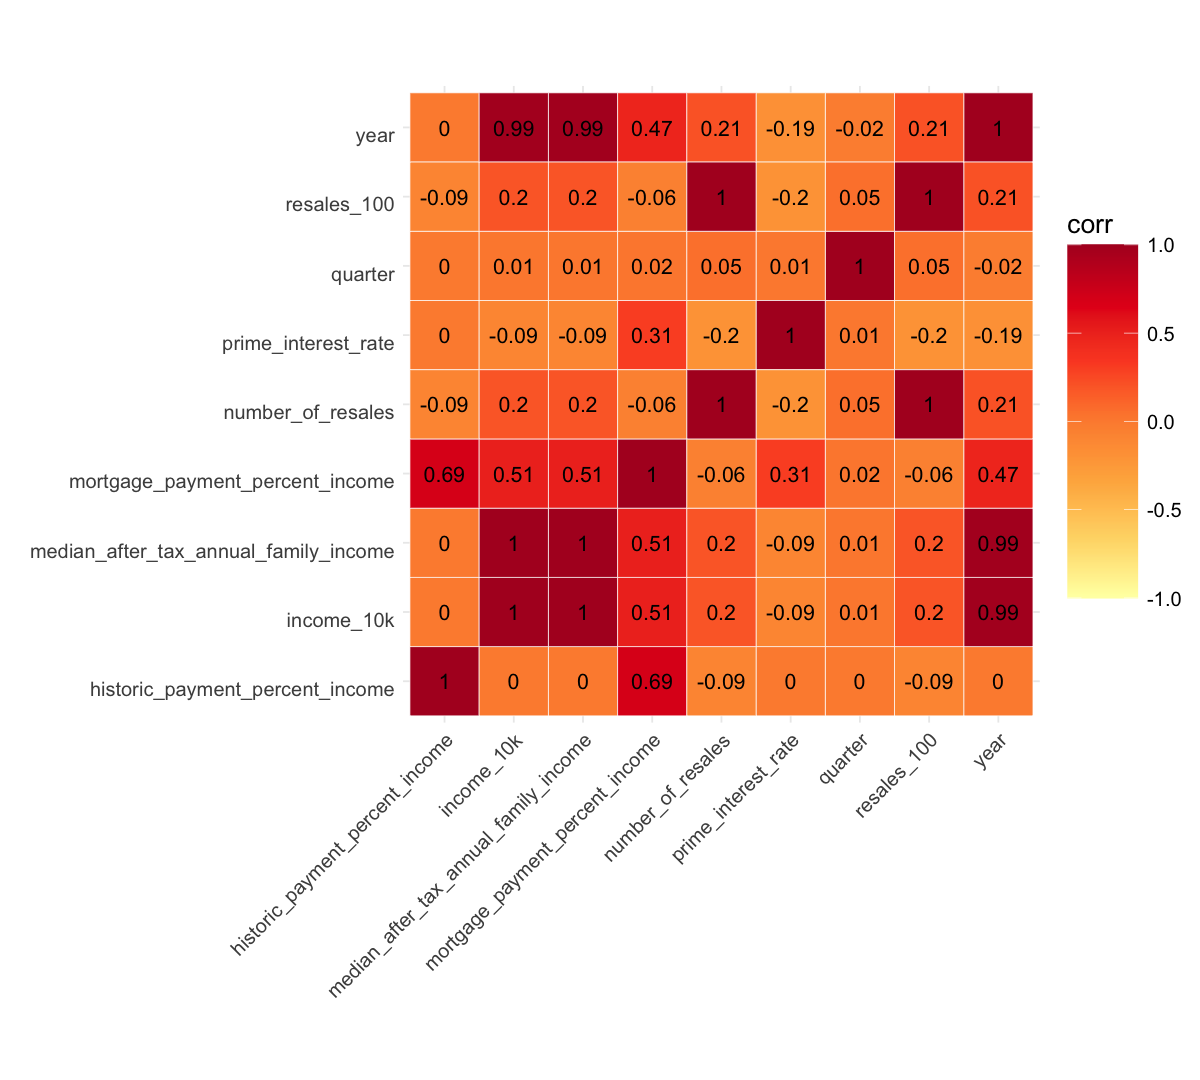
\includegraphics[width=0.65\textwidth]{figs/heatmap.png}
    \caption{Correlation Coefficient between numeric explanatory variables. }
    \label{fig:heatmap}
\end{figure}

The heatmap above clearly portrays that some of our variables are highly correlated with each other. The covariates 'year' and 'median\_after\_tax\_annual\_family\_income' exhibit a strong correlation. While this may suggest multicollinearity, 'year' serves as a time index. The strong correlations are likely due to the underlying time trends which indicates potential time dependence in the data.

\begin{figure}[H]
    \centering
    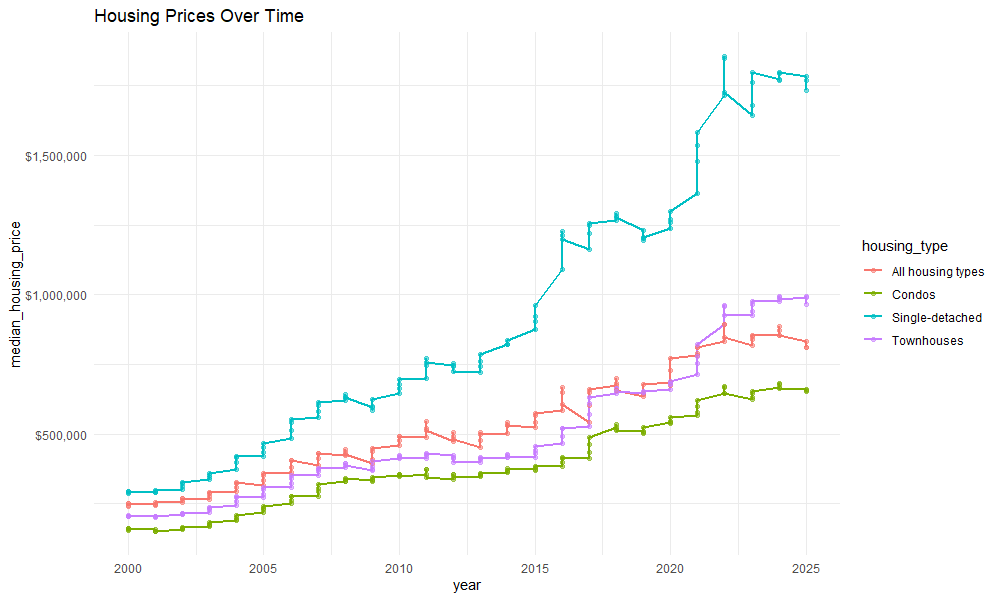
\includegraphics[width=0.75\textwidth]{figs/housingpriceslinegraph.png}
    \caption{Housing prices over time among different housing types.}
\end{figure}

The line plot shows a strong upward trend in median housing prices across all housing types. Single-detached houses consistently have the highest prices, followed by townhouses, while condos remain the least expensive. Price growth also seems to accelerate after 2015. \\

Since this is time series data, observations that are close in time are likely to be correlated. This suggests a potential violation of the independence assumption, as consecutive observations may not be independent.

\begin{figure}[H]
    \centering
    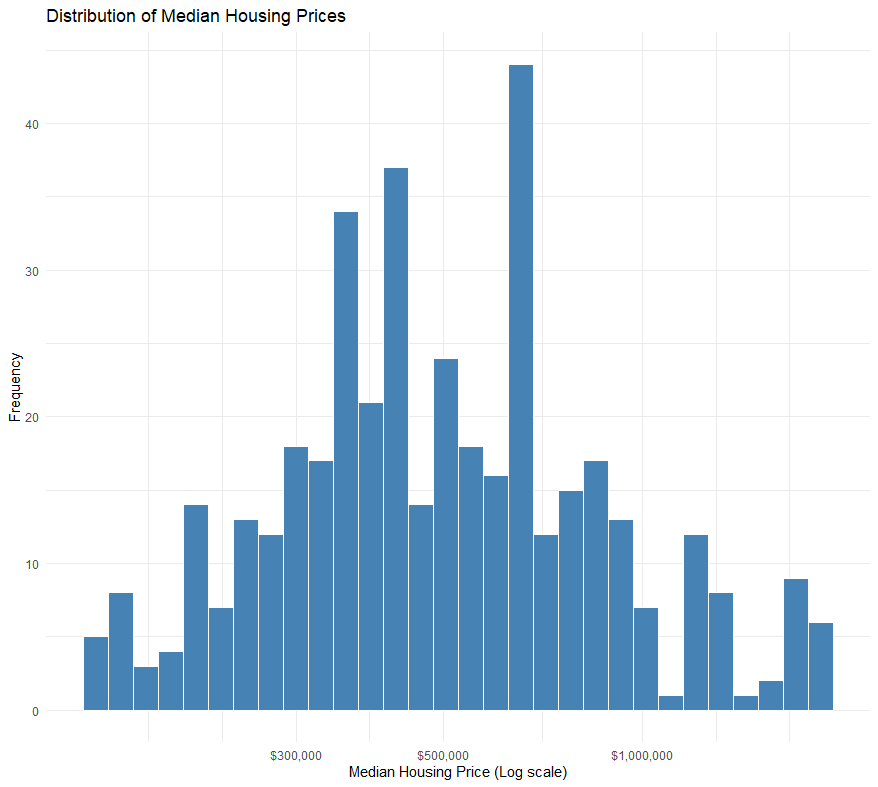
\includegraphics[width=0.6\textwidth]{figs/distribution.png}
    \caption{Distribution of log transformed Median Housing Prices}
\end{figure}

% TODO change it to bimodal and change discussion about it
The log-transformed distribution of median housing prices appears approximately symmetric but there is evidence of multiple peaks, suggesting a weakly bimodal distribution. While the log-transformation reduces the strong right-skewness present in the original data, some clustering remains across different price ranges. Overall, the transformation makes the data more suitable for regression analysis.

\section*{Statistical analysis}
We scaled some covariates to make interpreting the model easier, namely dividing \texttt{income} by 10000, and \texttt{resales} by 100.

\subsection*{Model Selection}
From initial checks, we see that \texttt{historic\_payment\_percent\_income} can be expressed as a linear combination of other covariates, so we will remove them in order to find VIF values. You may see appendix for the related R output for this part. \\

\begin{table}[H]
    \centering
    \small
    \begin{tabular}{lrrr}
        \toprule
        & GVIF & Df & GVIF\textasciicircum{}(1/(2*Df)) \\
        \midrule
        year & 85.068557 & 1 & 9.223262 \\
        quarter & 1.114402 & 1 & 1.055652 \\
        housing\_type & 20.780986 & 3 & 1.658101 \\
        prime\_interest\_rate & 3.185203 & 1 & 1.784714 \\
        income\_10k & 80.281888 & 1 & 8.960016 \\
        mortgage\_payment\_percent\_income & 8.075838 & 1 & 2.841802 \\
        resales\_100 & 4.851840 & 1 & 2.202689 \\
        \bottomrule
    \end{tabular}
    \caption{GVIF for the predictors in the reduced regression model after removing \texttt{historic\_payment\_percent\_income} due to multicollinearity.}
\end{table}

From the above, we see that \texttt{year}, \texttt{income\_10k}, \texttt{housing\_type} all have VIF values >10, suggesting multicollinearity as we previously pointed out during EDA. We will drop \texttt{year} as our research question seeks to find relationships between housing prices and economic variables like income. We also drop MPPI due to its mechanical relationship with price and interest rates as described in the technical notes from the BC Data Catalogue about our dataset.

\begin{table}[H]
    \centering
    \small
    \begin{tabular}{lrrr}
        \toprule
        Variable & GVIF & Df & GVIF\textasciicircum{}(1/(2*Df)) \\
        \midrule
        housing\_type & 4.264022 & 3 & 1.273415 \\
        income\_10k & 1.156558 & 1 & 1.075434 \\
        quarter & 1.011980 & 1 & 1.005972 \\
        prime\_interest\_rate & 1.159549 & 1 & 1.076823 \\
        resales\_100 & 4.602533 & 1 & 2.145352 \\
        \bottomrule
    \end{tabular}
    \caption{GVIF for the predictors after removing \texttt{year} and \texttt{mppi}.}
\end{table}

We observe that after removal of the two covariates, the VIF values have greatly improved below our rule-of-thumb value of 10, suggesting that we have dealt with the multicollinearity problem between our covariates. We compared four candidate subsets using Adjusted $R^2$ and Mallows' $C_p$ criteria to find a simpler model.

\begin{table}[H]
    \centering
    \small
    \begin{tabular}{rrrr}
        \toprule
        p\_params & SSRes & Cp & Adj\_R2 \\
        \midrule
        6 & 5.8831 & 6.83 & 0.9539540 \\
        7 & 5.8625 & 7.41 & 0.9540015 \\
        7 & 5.8671 & 7.72 & 0.9539658 \\
        8 & 5.8421 & 8.00 & 0.9540480 \\
        \bottomrule
    \end{tabular}
    \caption{Model comparison results for four candidate subsets using adjusted $R^2$ and Mallows' $C_p$.}
\end{table}

Our objective was to select the most parsimonious model, i.e., the simplest version that maintains high predictive accuracy without introducing bias.
As shown in the comparison table, the \textbf{Base Model} (including Housing Type, Income, and Prime Rate) achieved an \textbf{Adjusted $R^2$ of 0.9539}. Adding number of resales (\texttt{resales}) and seasonality (\texttt{quarter}) only increased the Adjusted $R^2$ by a negligible \textbf{0.0001}, suggesting these variables provide almost no additional explanatory power.\
Furthermore, the \textbf{Mallows' $C_p$} for the Base Model was \textbf{6.83}, which is close to the expected value ($k=7$). This indicates the model is unbiased and follows the \textbf{Principle of Parsimony}.
Therefore, the Base Model was selected as the final representation.

\begin{table}[H]
    \centering
    \small
    \begin{tabular}{lrrr}
        \toprule
        & GVIF & Df & GVIF\textasciicircum{}(1/(2*Df)) \\
        \midrule
        housing\_type & 1.000000 & 3 & 1.000000 \\
        income\_10k & 1.008783 & 1 & 1.004382 \\
        prime\_interest\_rate & 1.008783 & 1 & 1.004382 \\
        \bottomrule
    \end{tabular}
    \caption{GVIF analysis on final model, showing low likelihood of multicollinearity.}
\end{table}

\begin{table}[H]
    \centering
    \small
    \begin{tabular}{lrrrrrr}
        \toprule
        term & estimate & std.error & statistic & p.value & conf.low & conf.high \\
        \midrule
        (Intercept) & 11.348 & 0.0326 & 348.0 & 0 & 11.3 & 11.4 \\
        housing\_typeCondos & -0.340 & 0.0168 & -20.3 & 0 & -0.373 & -0.307 \\
        housing\_typeSingle-detached & 0.452 & 0.0168 & 27.0 & 0 & 0.419 & 0.485 \\
        housing\_typeTownhouses & -0.104 & 0.0168 & -6.18 & 0 & -0.137 & -0.0708 \\
        income\_10k & 0.278 & 0.00360 & 77.2 & 0 & 0.271 & 0.285 \\
        prime\_interest\_rate & -0.0283 & 0.00387 & -7.32 & 0 & -0.0359 & -0.0207 \\
        \bottomrule
    \end{tabular}
    \caption{Coefficient estimates and 95\% confidence intervals for the final model.}
\end{table}

\begin{table}[H]
    \centering
    \small
    \begin{tabular}{rrrrrrrrr}
        \toprule
        r.squared & adj.r.squared & sigma & statistic & p.value & df & logLik & AIC & BIC \\
        \midrule
        0.955 & 0.954 & 0.120 & 1704.0 & 7.25e-270 & 5 & 291.0 & -567.0 & -539.0 \\
        \bottomrule
    \end{tabular}
    \caption{Overall fit statistics for the final regression model.}
\end{table}

The residuals-versus-fitted plot (Figure 4 Plot 1) has points randomly scattered across the plot, which suggests a linear plot is appropriate, and there is a small amount of heteroscedasticity, shown by the overall increase in the spread of residuals at higher fitted values, which still roughly supports the constant-variance assumption.\\
The Q-Q residuals plot (Figure 4 Plot 2) closely follows a fairly straight line, with the trend only deviating slightly at the extreme tails, meaning the assumption of normality is unlikely violated.\\
The scale-location plot (Figure 4 Plot 3) supports the residuals-versus-fitted plot, as the standardized residuals are relatively horizontal, but has a slight increase at higher fitted values, so the variance is stable but a small amount of heteroscedasticity.\\
The residuals-versus-leverage plot (Figure 4 Plot 4) shows that none of the of observations exceed Cook's distance, meaning there are no strong outliers.\\
Overall, these plots suggest roughly constant variance and normality with no influential observations, although there is small non-constant spread at the extreme fitted values.

\begin{figure}[H]
    \centering
    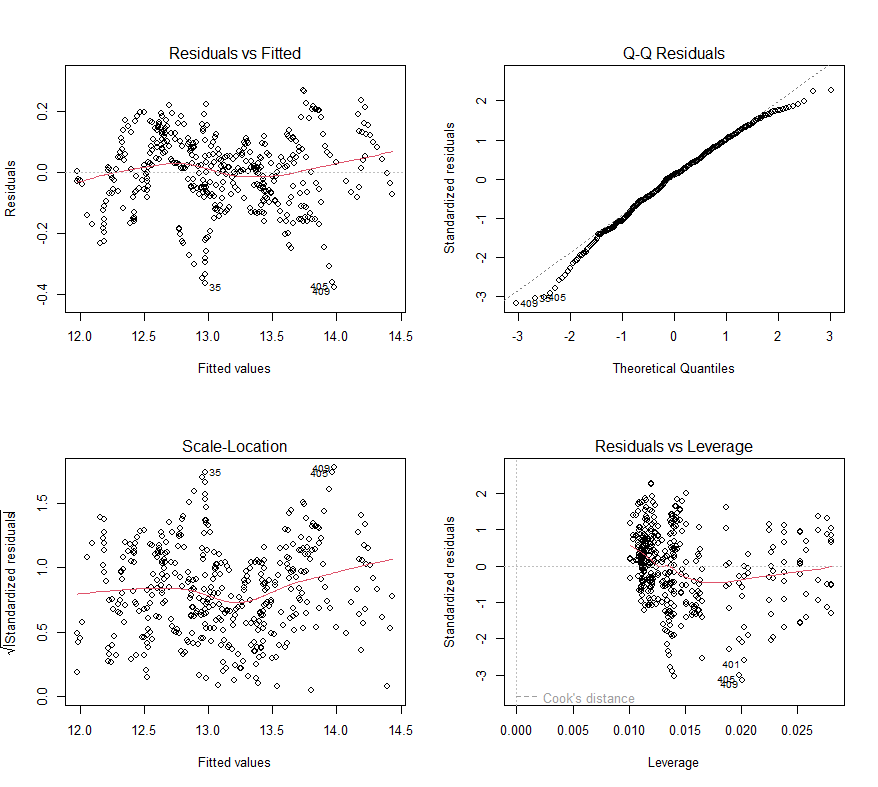
\includegraphics[width=0.65\textwidth]{figs/varianceassumptionplots.png}
    \caption{Diagnostic plots for the final linear regression model.}
\end{figure}
\clearpage

The residuals-versus-income plot (Figure 5) shows some non-constant variance at the extreme lower and upper ends. The residuals-versus-prime-interest-rate plot shows a more even spread, supporting the constant variance assumption for this predictor. The residuals-housing-type boxplots show a similar spread across categories.

\begin{figure}[H]
    \centering
    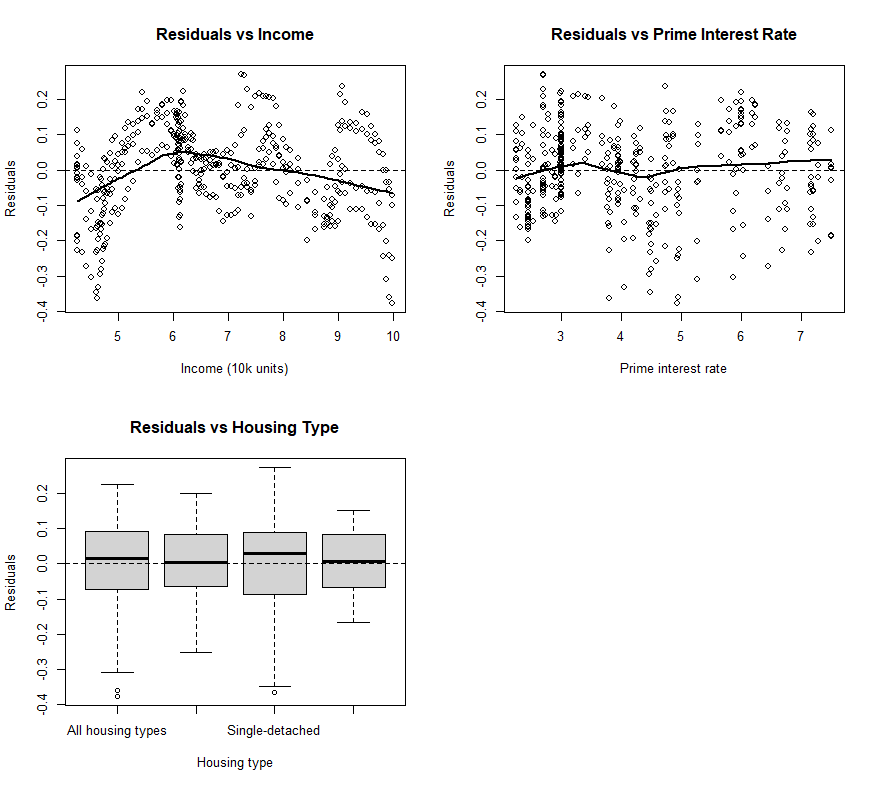
\includegraphics[width=0.6\textwidth]{figs/2by2.png}
    \caption{Residuals plotted against covariates in the final linear regression model.}
\end{figure}

Lastly, the sequential residual plot (Figure 6) reveals a wave-like structure. This suggests that the errors are not fully independent over time, indicating that the current model may be inadequate for capturing temporal autocorrelation.

\begin{figure}[H]
    \centering
    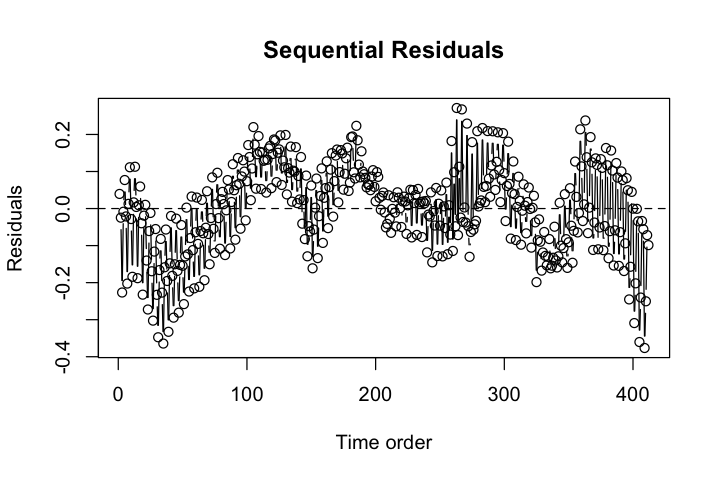
\includegraphics[width=0.6\textwidth]{figs/seqresids.png}
\caption{Sequential residual plot for the final linear regression model.}
\end{figure}
\clearpage

\section*{Discussion}
Using multiple linear regression, we derived the following model to describe the relationship between macroeconomic factors and housing prices in Metro Vancouver:
\begin{equation*}
    \begin{aligned}
        \log(\widehat{\text{median\_housing\_price}}) = 11.348 &- 0.340 \cdot I\{\text{housing\_typeCondos}\} + 0.452 \cdot I\{\text{housing\_typeSingle-detached}\} \\
        &- 0.104 \cdot I\{\text{housing\_typeTownhouses}\} + 0.278(\text{income\_10k}) \\
        &- 0.0283(\text{prime\_interest\_rate})
    \end{aligned}
\end{equation*}

The fitted model observes that a higher median family income is associated with higher median housing prices, whereas higher prime interest rates are associated with lower median housing prices. Furthermore, we notice a distinct hierarchy among housing types. When holding other factors constant, single-detached homes have the highest expected prices, followed by townhouses, the regional average (``All Housing Types''), and finally condos.\\

Because we log-transformed the response variable to stabilize variance, the coefficients correspond to multiplicative changes rather than linear dollar changes. For example, the income coefficient of 0.278 implies that for every \$10,000 increase in median annual after-tax family income, the median housing price is associated with an approximately \textbf{32\% increase} ($e^{0.278} \approx 1.32$). Similarly, a 1\% increase in the prime interest rate is associated with an approximately \textbf{2.8\% decrease} in price ($e^{-0.0283} \approx 0.972$). All coefficients proved to be statistically significant ($p < 0.001$), and their 95\% confidence intervals did not cross zero, as seen in Table 7. Consequently, we can be fairly confident in these estimated associations. \\

The appropriateness of our model remains a subject for debate. Our model explains roughly 95.4\% of the variation in log-median housing prices. Diagnostics in Figure 4 (Residuals vs. Fitted and Q-Q plots) generally support the assumption of constant variance and normality. This is further supported by the residual-versus-interest rate plot in Figure 5.  All of these results support the use of linear regression as an appropriate model for this dataset. \\

On the other hand, the residuals-versus-income plot (Figure 5) showed concerning trends at the extreme ends, suggesting slight heteroscedasticity. Additionally, the sequential residual plot (Figure 6) reveals a clear ``wave-like'' pattern, which signals a \textbf{lack of independence} among sequential observations. This makes some sense, as our current model does not directly factor in time. This suggests the presence of temporal autocorrelation, where housing prices in one quarter are heavily dependent on prices in previous quarters. This is logical, as housing markets are influenced by broader economic and political cycles (e.g., the 2008 recession or recent downturns) that a simple linear model cannot fully capture.\\

Furthermore, concerns of multicollinearity limited the covariates we could include. We removed \texttt{YEAR} due to its high collinearity with median income; including both would have destabilized the model. We also consciously excluded \texttt{number\_of\_resales} from the final model, as its addition did not significantly improve predictive accuracy or explanatory power, though this leads us to reflect on whether we fully addressed the resale component of our initial research question. \\

In terms of the data itself, this study is observational, meaning we can make only associative determinations, not causal ones. Additionally, the study utilizes aggregate quarterly measures; this implies that variables such as median housing price and median family income are identical across rows within the same year and quarter. Consequently, household-level variation cannot be determined, and assessing the distribution or skew of housing prices within a single quarter remains a challenge. \\

In the future, we would prefer to choose a model more focused on time-series data and the non-linear relations between housing price and our covariates. It would also be helpful to have in this new non-linear model other market related variables un-related to housing. For example, it may be interesting to see how inflation, or recession indicators affect the median housing price. \\

In summary, while our model is effective at capturing the primary associations between median housing prices, family income, and interest rates, it fails to fully account for hidden temporal cycles. The nature of the data leads to slight violations of the constant variance and independence assumptions underlying the linear regression framework.

\newpage
\section*{Appendix}
\subsection*{R Model Selection: Linear Combination Output}
\begin{small}
    \begin{verbatim}
    Model :
    log(median_housing_price) ~ year + quarter + housing_type + prime_interest_rate + 
        income_10k + mortgage_payment_percent_income + historic_payment_percent_income + 
        resales_100

    Complete :
                                    (Intercept)   year          quarter      
    historic_payment_percent_income  676846/14603             0             0
                                    housing_typeCondos housing_typeSingle-detached
    historic_payment_percent_income -435524/33949          12877/472              
                                    housing_typeTownhouses prime_interest_rate
    historic_payment_percent_income -132947/38534                      0      
                                    income_10k    mortgage_payment_percent_income
    historic_payment_percent_income             0             0                  
                                    resales_100  
    historic_payment_percent_income             0
    \end{verbatim}
\end{small}

\section*{Statement of AI Use}
We used AI to help create the latex document, format it, and transcribe tables from our jupyter notebook to the more formattable latex format before creating our PDF for submission.

Prompt: Here is my jupyter notebook, please transcribe all data frames and tables over to a copy-pasteable latex format exactly as is. Do not do any other work, this is to help avoid redundant work on our end purely for transcription.

\section*{Reference}
Housing Affordability for Homeowners in B.C. Technical Note,
\href{https://catalogue.data.gov.bc.ca/dataset/b-c-housing-affordability/resource/f8153a37-f18d-4d4e-bbe6-77f648bc1f31=}{\underline{link}}
\end{document}
